\documentclass[fontsize=12pt, paper=a4, abstract=true]{scrartcl}
\usepackage{theiss}     % loads custom template

%% TITLE INFO %%
\author{Name of Author}
\date{Month DD, YYYY}

\newcommand{\TitleOfEssay}{Title of Essay}
\newcommand{\StudentID}{1234567}
\newcommand{\NameOfModule}{MBB--MA--XXX--Y: Name of Module}
\newcommand{\NameOfSeminar}{SX: Name of Seminar}
\newcommand{\RunningHead}{
    \MakeUppercase{Running Head}    % max. 50 characters
    }

\hypersetup{
    pdftitle=\TitleOfEssay,
    pdfauthor=\theauthor,
    bookmarksopenlevel=1
    }

%% BIB-FILE(S) %%
\addbibresource{bibliography/example.bib}

%% BEGINNING OF DOCUMENT %%
\StopCensoring
\begin{document}

%% FRONTMATTER %%
\begin{center}
    {\onehalfspacing
        \vspace*{2mm}
        {\LARGE
            \TitleOfEssay\\
        }
        \vspace{5mm}

        {\large
            \theauthor\\
        }

        Student ID: \StudentID\\
        \vspace{5mm}

        {\large
            \NameOfSeminar\\
        }

        \NameOfModule\\
        \vspace{5mm}

        \thedate
    }
\end{center}
% https://apastyle.apa.org/instructional-aids/abstract-keywords-guide.pdf

\vspace{2mm}
\noindent\hfil\rule{.95\textwidth}{.5pt}\hfil
%
\begin{abstract}
    {\onehalfspacing\justifying
        \noindent
        \lipsum[1-1]    % max. 250 words!

        \vspace{2mm}
        \textbf{Keywords:} keyword 1, keyword 2, keyword 3
    }
\end{abstract}
%
\noindent\hfil\rule{.95\textwidth}{.5pt}\hfil\\
\vspace{2mm}
%\vspace{2mm}
\noindent\hfil\rule{.95\textwidth}{.5pt}\hfil\\
\vspace{2mm}

%% MAIN TEXT %%
\begin{multicols}{2}
    %% SECTION 1 %%
\section*{Heading}

This is a sample reference \citep{Herzog2016TimeSlices}. And here is another one \citep{Fekete2018CritiqueDiscretePerception}.
    %% SUBSECTION 1.1 %%
\subsection*{Subheading.}

\lipsum[1]


%% SUBSECTION 1.1.1 %%
\subsubsection*{Subheading.}

\lipsum[2]


%% SUBSECTION 1.1.2 %%
\subsubsection*{Subheading.}

\lipsum[3]
    %% SUBSECTION 1.2 %%
\subsection*{Subheading.}

\lipsum[4]


%% SUBSECTION 1.2.1 %%
\subsubsection*{Subheading.}

\lipsum[5]


%% SUBSECTION 1.2.2 %%
\subsubsection*{Subheading.}

\lipsum[6]
\end{multicols}

%% ADD REFERENCES %%
\emergencystretch=2em           % prevents 'overfull hbox' errors
\RedeclareSectionCommand[
  runin=false,               % unchanged
  afterindent=true,          % unchanged
  beforeskip=\baselineskip,  % unchanged
  afterskip=.5\baselineskip  % add vertical space after heading
]{section}

\printbibliography           % print references


%% ADD DECLARATION OF AUTHORSHIP %%
%% DECLARATION %%
\newpage
\justifying
\section*{Declaration of Authorship}

\subsection*{Authorship and academic integrity.}

I hereby declare that I have written this report independently and have not used any other than the specified resources. The parts of the work that are taken from other works in wording or meaning are indicated by references and sources. This also applies to drawings, sketches, example scripts, and the like.

\begin{figure}[h]
    \hfill\begin{minipage}{4cm}
        \centering
        \censorbox{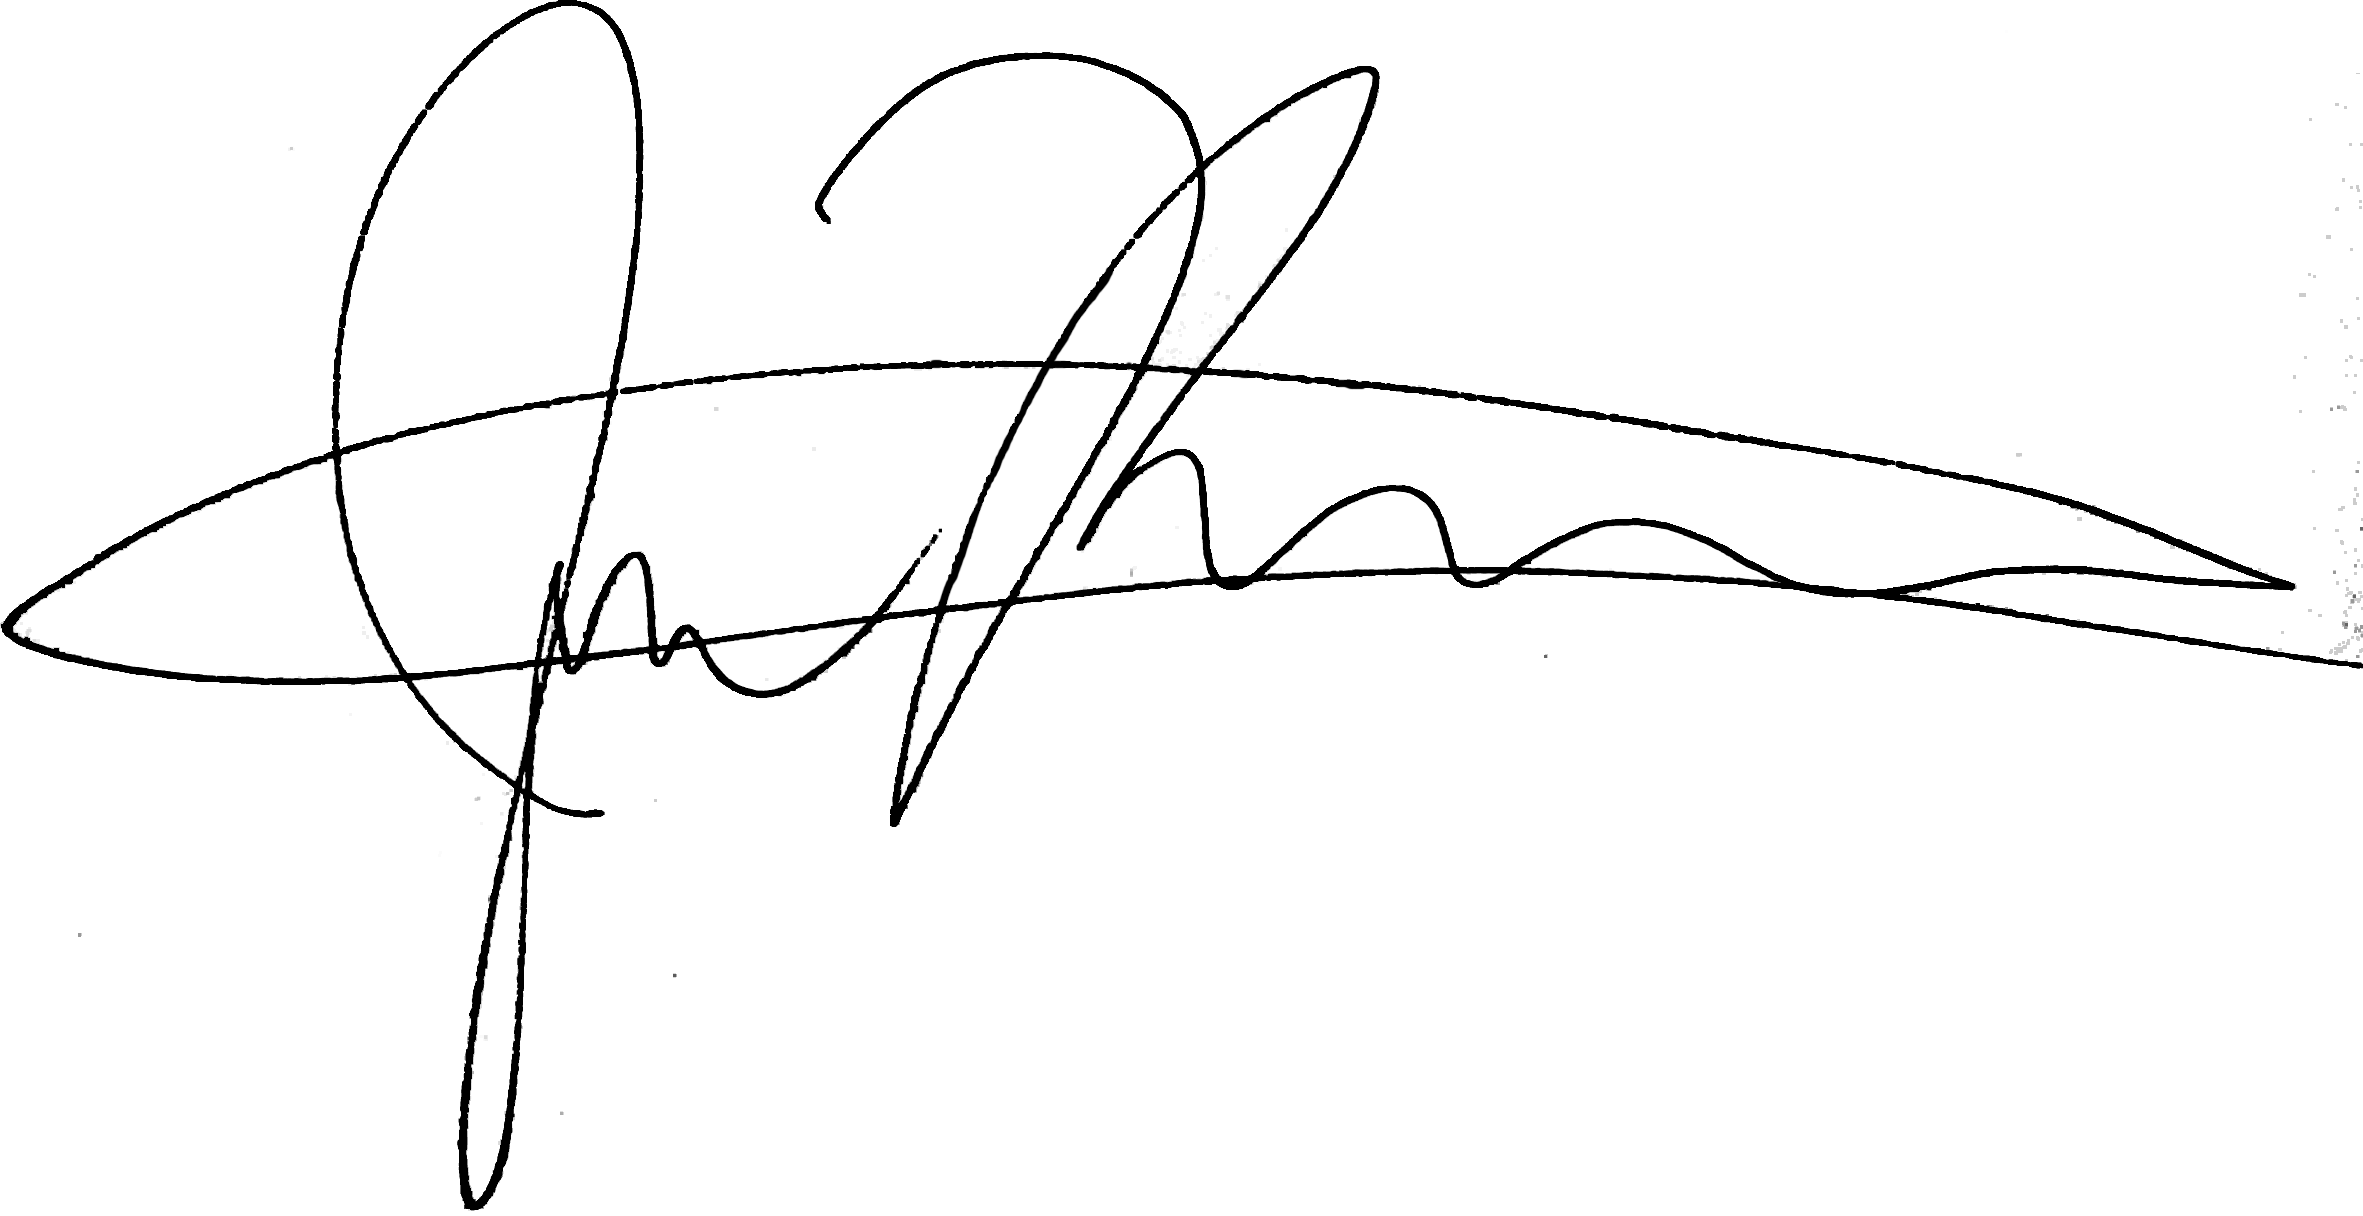
\includegraphics[width=4cm]{sample-signature}}
        \textsc{Author Name}
    \end{minipage}\hspace{1cm}
\end{figure}

\end{document}
%% END OF DOCUMENT %%